\documentclass[11pt,a4paper,twoside]{article}
\usepackage[utf8]{inputenc}
\usepackage[T1,T2A]{fontenc}
\usepackage[english.ancient,russian.ancient]{babel}
\usepackage{graphicx}
\usepackage{array}
\usepackage[doi]{samgtu-bib}
\usepackage{mdtt-samara}
\usepackage{mathtools}
\mathtoolsset{showonlyrefs}
\usepackage{desclist}
\usepackage{euscript}
\usepackage{mathrsfs} 
\usepackage{multicol}
\usepackage{mathrsfs}
\usepackage{cite}
\usepackage{qrcode}
\allowdisplaybreaks[4]
\usepackage[nodayofweek]{datetime}

\renewcommand{\JournalYear}{2017}
\renewcommand{\JournalVolume}{21}
\renewcommand{\JournalNumber}{x}

\newcommand{\totop}[1]{\raisebox{6pt}[1pt][2pt]{#1}}
\graphicspath{{./00PIC/}}

\FirstPage{1}
\LastPage{x}

\pdfcrop
%\draft

\begin{document}

\rutitle{Настройка Jenkins}

\Section[n]{Первоначальная настройка}
\begin{figure}[h!]
    \centering
    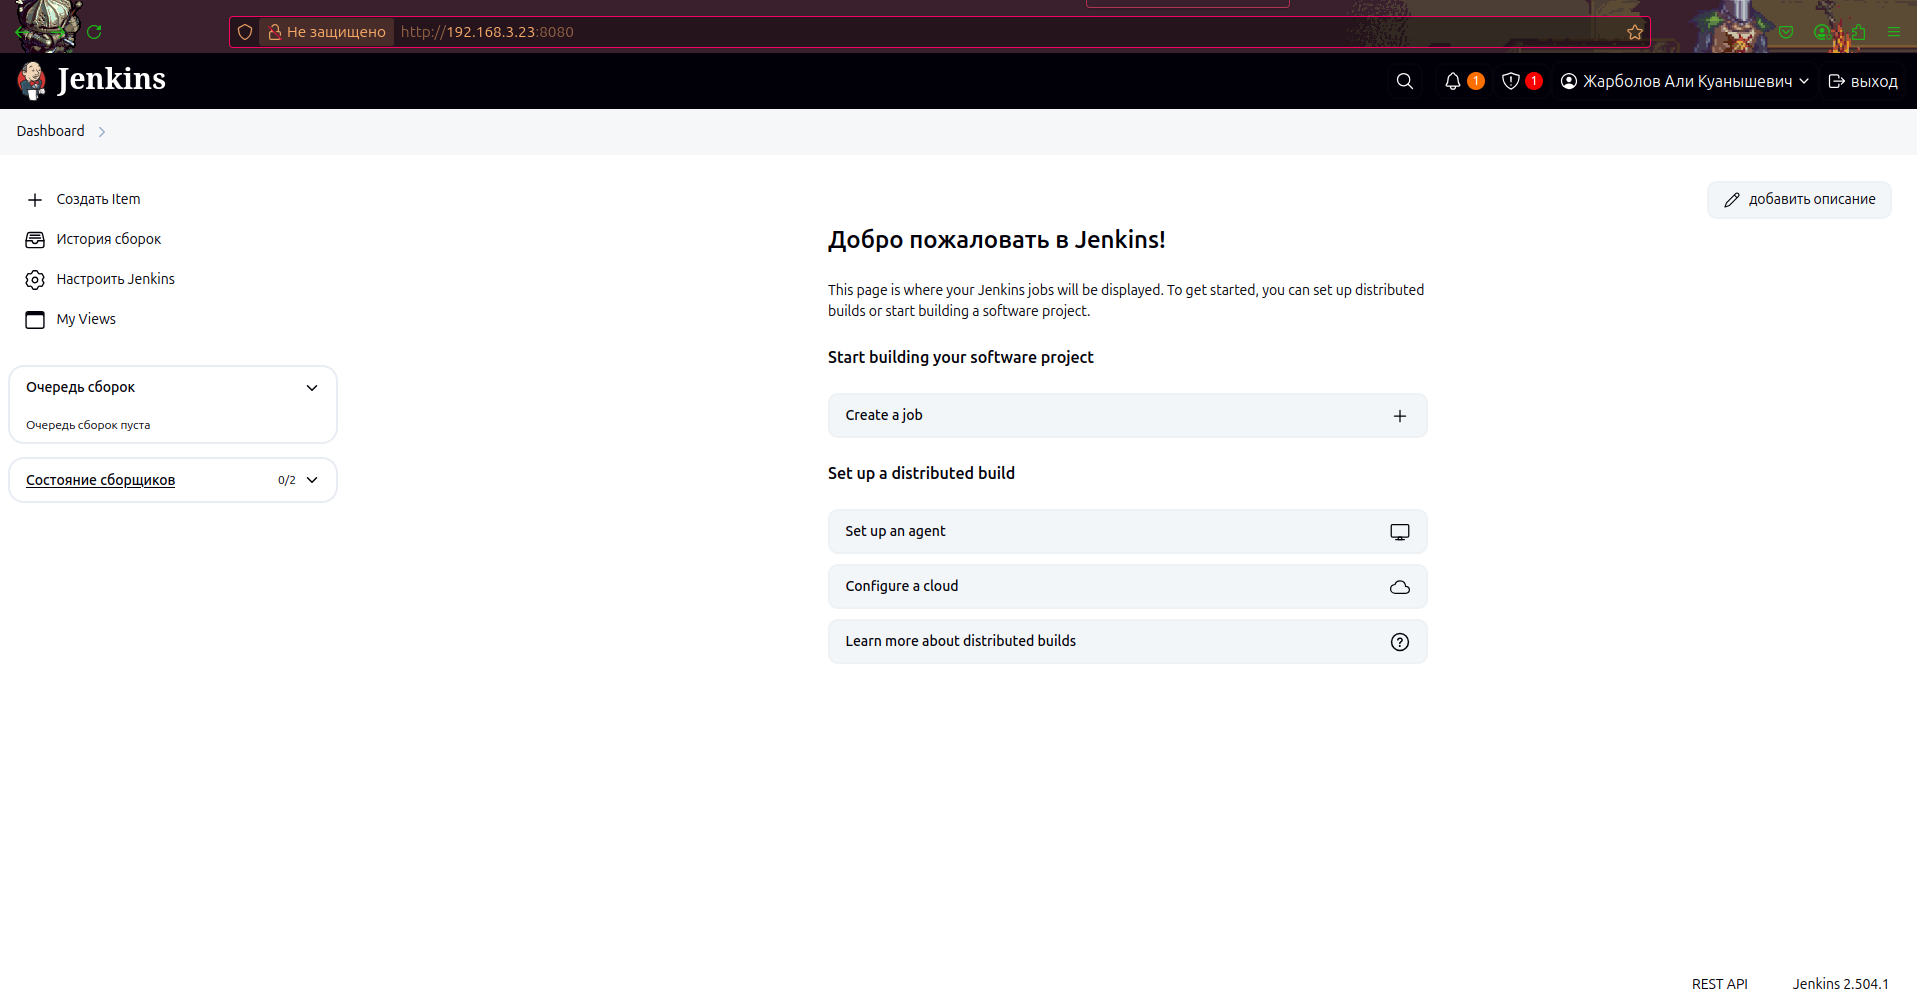
\includegraphics[width=0.5\linewidth]{pic/1.png}
    \caption{Стартовая страница}
    \label{fig:enter-label}
\end{figure}
\begin{figure}[h!]
    \centering
    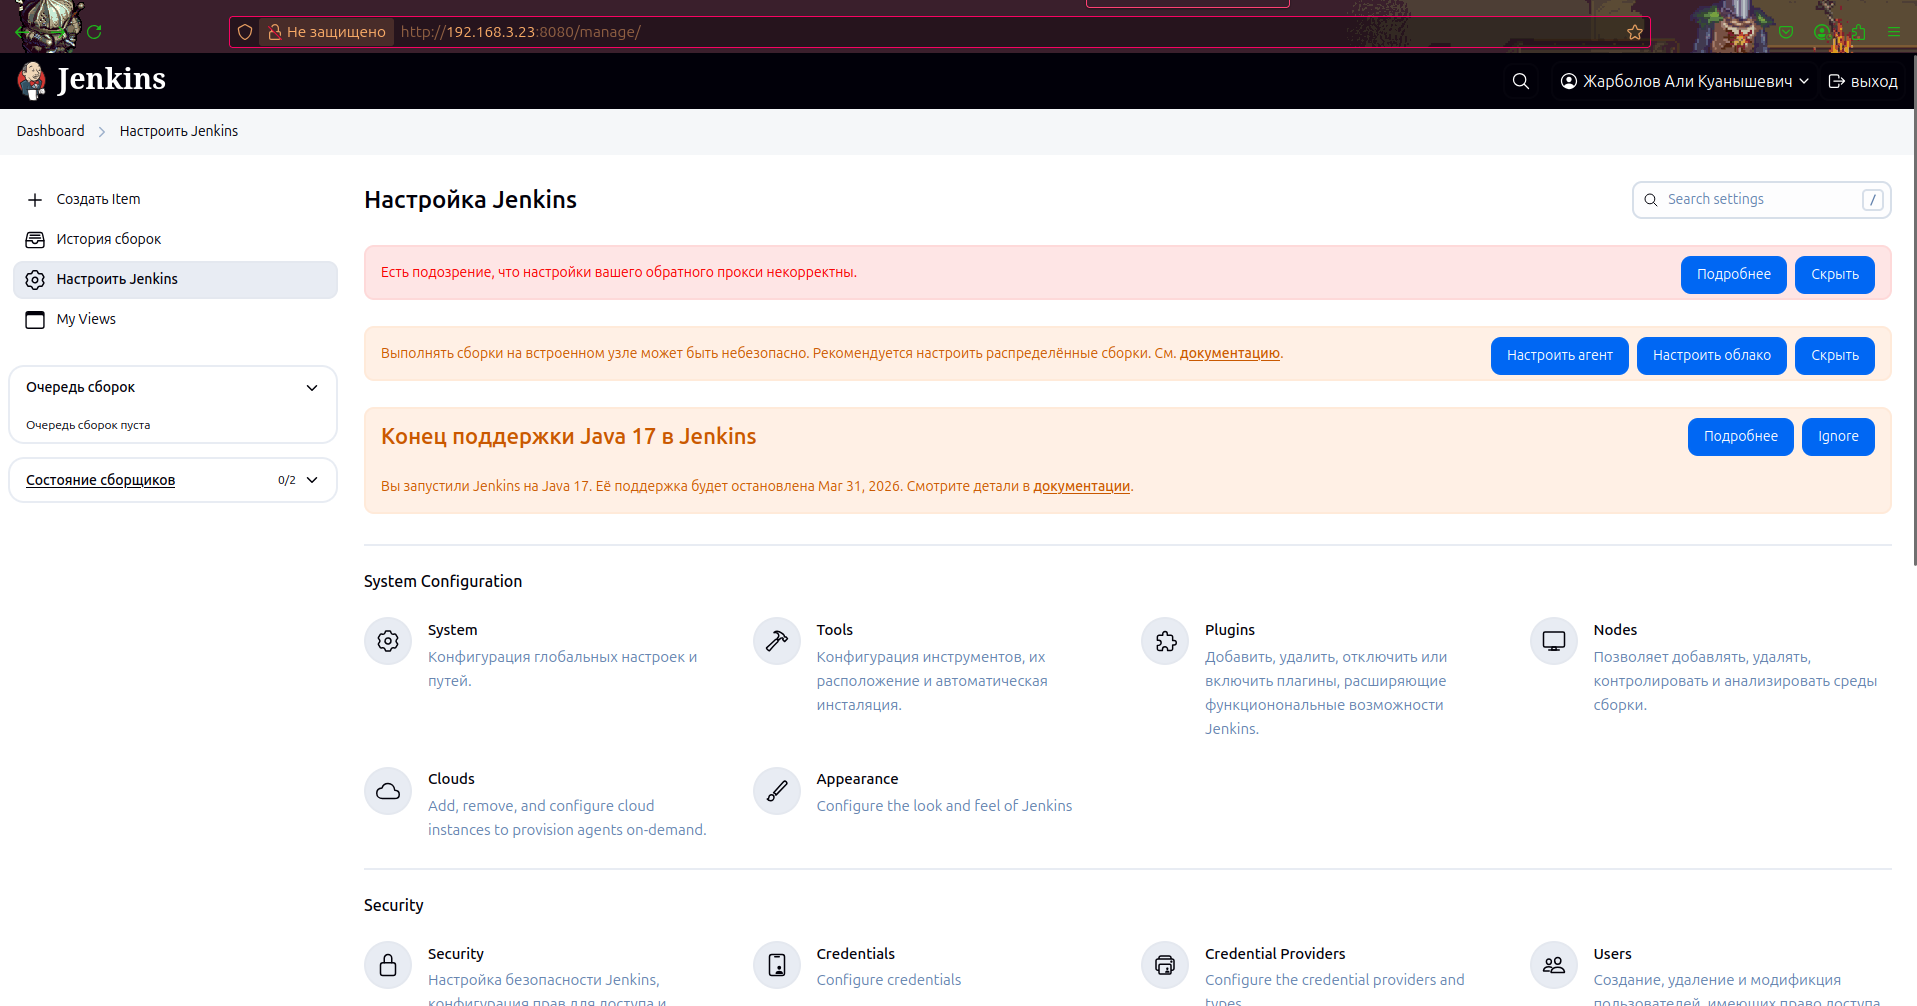
\includegraphics[width=0.5\linewidth]{pic/2.png}
    \caption{Заходим в настройки}
    \label{fig:enter-label}
\end{figure}

\begin{figure}[h!]
    \centering
    
\includegraphics[width=0.5\linewidth]{pic/3.png}
    \caption{Меняем узел}
    \label{fig:enter-label}
\end{figure}

\begin{figure}[h!]
    \centering
    
\includegraphics[width=0.5\linewidth]{pic/4.png}
    \caption{Настраиваем}
    \label{fig:enter-label}
\end{figure}

\begin{figure}[h!]
    \centering
    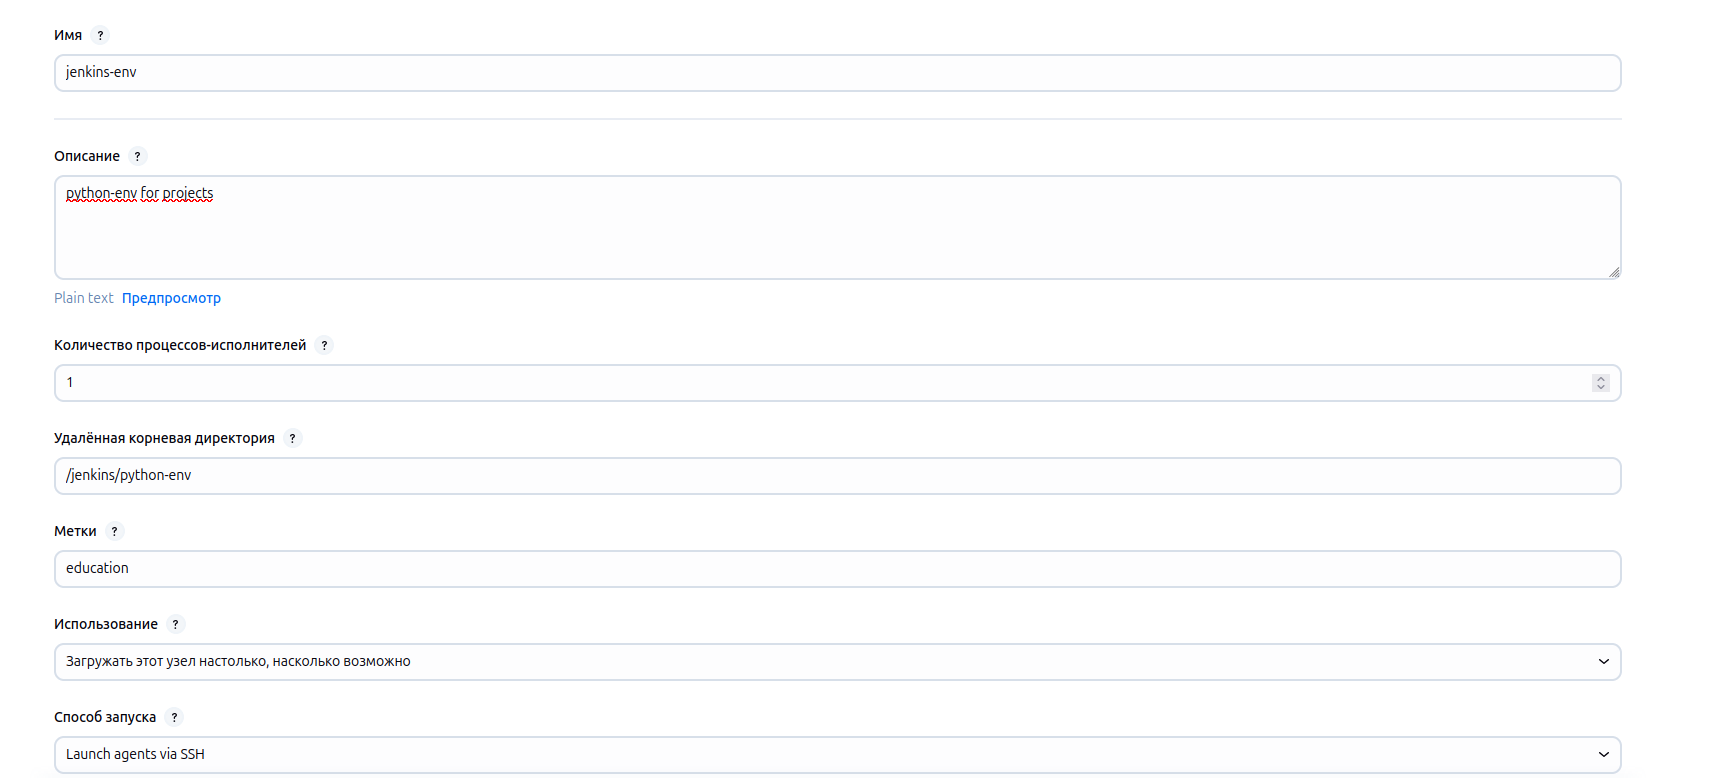
\includegraphics[width=0.5\linewidth]{pic/5.png}
    \caption{Настраиваем}
    \label{fig:enter-label}
\end{figure}

\begin{figure}[h!]
    \centering
    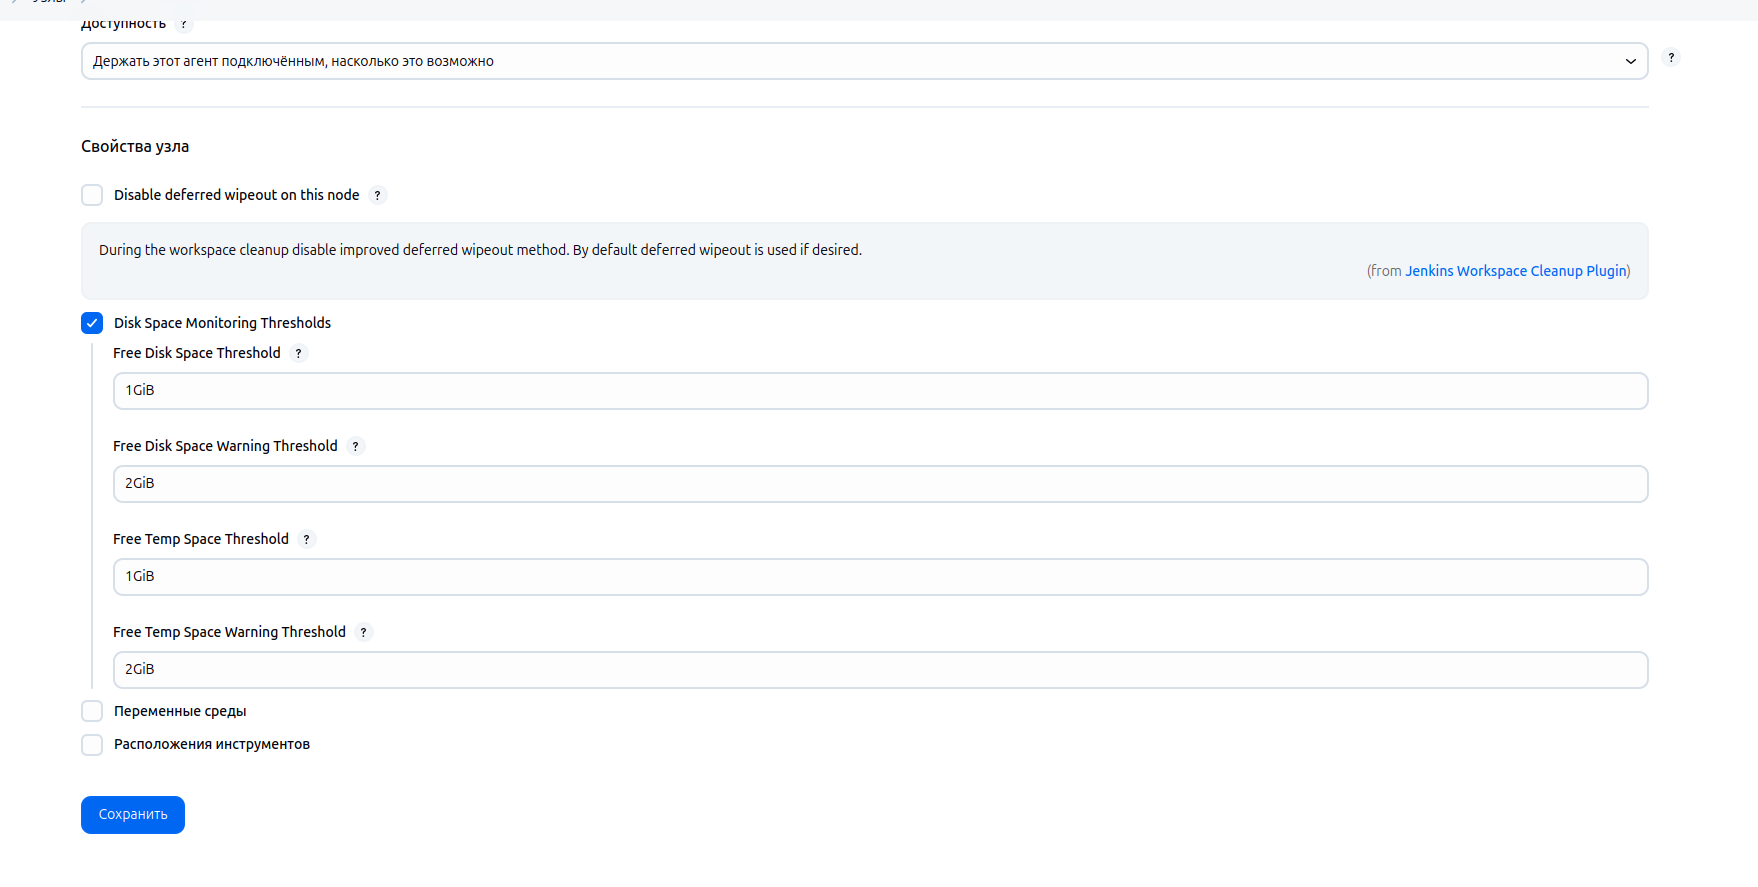
\includegraphics[width=0.5\linewidth]{pic/6.png}
    \caption{Настраиваем}
    \label{fig:enter-label}
\end{figure}

\begin{figure}[h!]
    \centering
    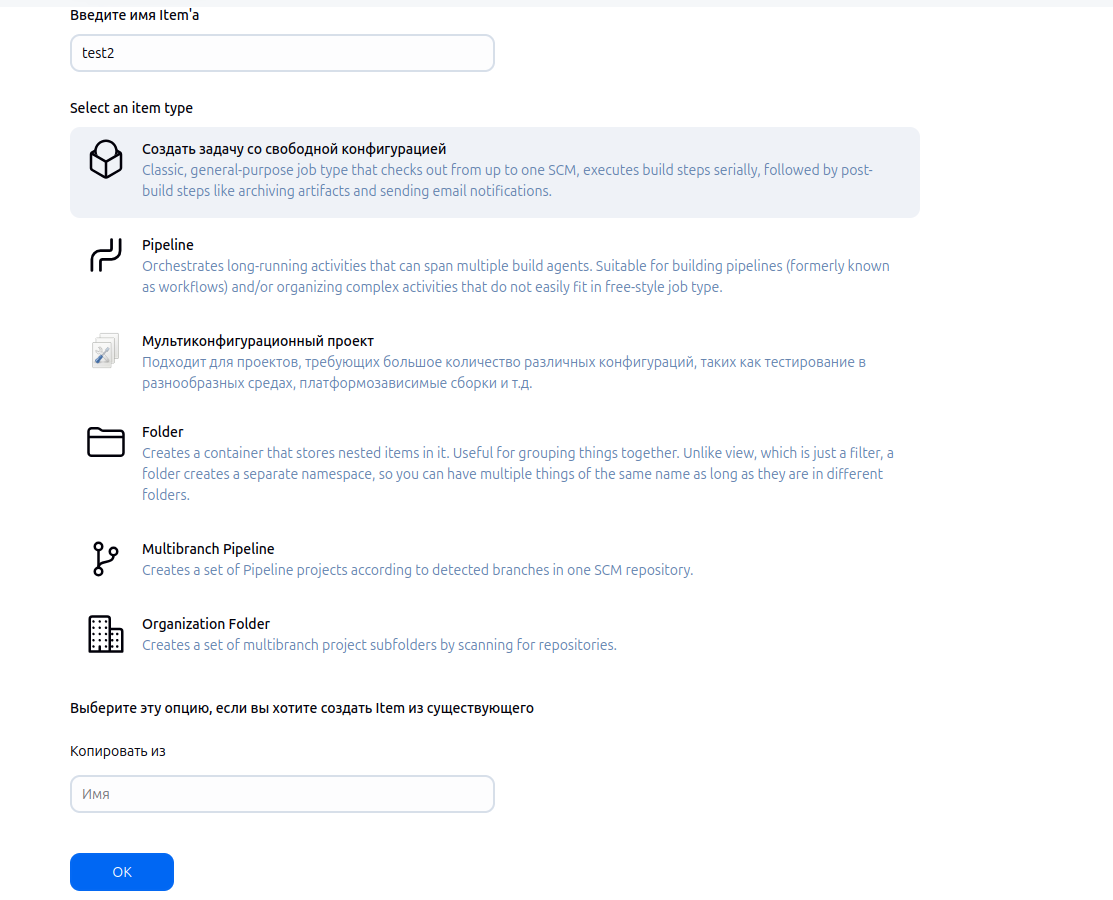
\includegraphics[width=0.5\linewidth]{pic/8.png}
    \caption{Создаем новый item}
    \label{fig:enter-label}
\end{figure}
\newpage
\Section[n]{Циклы} 
Выставляем в параметрах команды shell. Пишем скрипт, который будет исполнять система. 
\begin{verbatim}
python3 -m venv ./my_env # создаем окружение python
. ./my_env/bin/activate  # активируем 
cd /var/lib/jenkins/workspace/download/model		 	
python3 -m ensurepip --upgrade
pip3 install setuptools
pip3 install -r requirements.txt  # установка зависимостей
python3 ./download.py
#-----------------------
echo "Start train model"	   
python3 ./train_model.py > best_model.txt 
#------------------------   
export BUILD_ID=dontKillMe         
export JENKINS_NODE_COOKIE=dontKillMe
path_model=$(cat best_model.txt) 
mlflow models serve -m $path_model -p 5003 --no-conda & 
#------------------------
curl http://192.168.3.23:8080/invocations \
-H"Content-Type:application/json"  --data '{"inputs": \
[[ -1.275938045, -1.2340347 , -1.41327673,  0.76150439,\
2.20097247, -0.410937195,  0.58931542,  0.1135538,  0.58931542]]}'
pipeline {
    agent any

    stages {
        stage('Download') {
            steps {
                
                build job: 'download'
            }
        }
        
        stage ('Train') {
            
            steps {
                build job: 'train_model'
            
            }
        }
        
        stage ('Deploy') {
            steps {
                build job: 'deploy'
            }
        }
        
        stage ('Status') {
            steps {
                build job: 'healthy'
            }
        }
    }
}
\end{verbatim}
В файл requirements.txt важно записать следующие, т.к. сервер требует тонкой настройки.
\begin{verbatim}
joblib==1.2.0
scikit_learn==1.2.2 --no-binary=scikit-learn
mlflow==2.3.1
pandas==1.5.3 --no-binary=pandas
numpy==1.21.6 --no-binary=numpy
\end{verbatim}
Далее создаём директорию, которую будет запускать jenkins. Для этого надо организовать папку download. Создаём её на нашем компьютере вместе с исполняемыми файлами download.py и train\_model.py. Их код можно посмотреть в гитхабе. 

Важно копировать файловую структуру из скрипта. Когда файл будет создан, выгружаем его на сервер через scp.
\begin{verbatim}
    scp -P NNNN -r \home\user\download / 
    user@192.168.3.23:\var\lib\jenkins\workspace 
\end{verbatim}
Запускаем новую задачу. 
\begin{figure}
    \centering
    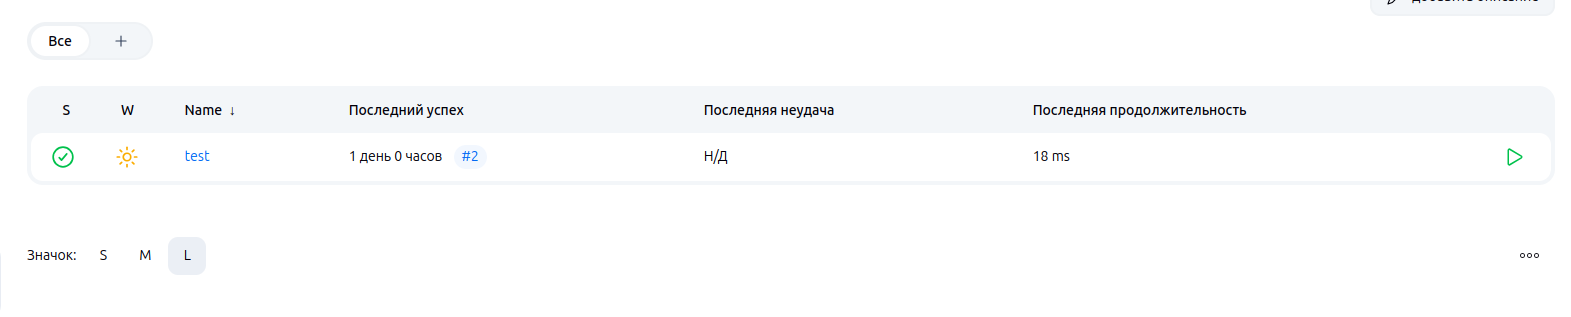
\includegraphics[width=0.5\linewidth]{pic/10.png}
    \caption{Рабочий запуск}
    \label{fig:enter-label}
\end{figure}
\end{document}
